%%%%%%%%%%%%%%%%%%%%%%%%%%%%%%%%%%%%%%%%%
% Short Sectioned Assignment
% LaTeX Template
% Version 1.0 (5/5/12)
%
% This template has been downloaded from:
% http://www.LaTeXTemplates.com
%
% Original author:
% Frits Wenneker (http://www.howtotex.com)
%
% License:
% CC BY-NC-SA 3.0 (http://creativecommons.org/licenses/by-nc-sa/3.0/)
%
%%%%%%%%%%%%%%%%%%%%%%%%%%%%%%%%%%%%%%%%%

%----------------------------------------------------------------------------------------
%	PACKAGES AND OTHER DOCUMENT CONFIGURATIONS
%----------------------------------------------------------------------------------------

\documentclass[paper=a4, fontsize=10pt]{article} % A4 paper and 11pt font size
\usepackage[a4paper,left=1.5cm,right=1.5cm,top=.25cm]{geometry}

\usepackage[T1]{fontenc} % Use 8-bit encoding that has 256 glyphs
\usepackage[english]{babel} % English language/hyphenation
\usepackage{amsmath,amsfonts,amsthm} % Math packages
\usepackage{epsfig}
\usepackage{sectsty} % Allows customizing section commands
\allsectionsfont{\centering \normalfont\scshape} % Make all sections centered, the default font and small caps
\usepackage{wrapfig}

\usepackage{fancyhdr} % Custom headers and footers
\pagestyle{fancyplain} % Makes all pages in the document conform to the custom headers and footers
\fancyhead{} % No page header - if you want one, create it in the same way as the footers below
\fancyfoot[L]{} % Empty left footer
\fancyfoot[C]{} % Empty center footer
\fancyfoot[R]{\thepage} % Page numbering for right footer
\renewcommand{\headrulewidth}{0pt} % Remove header underlines
\renewcommand{\footrulewidth}{0pt} % Remove footer underlines
\setlength{\headheight}{13.6pt} % Customize the height of the header

\numberwithin{equation}{section} % Number equations within sections (i.e. 1.1, 1.2, 2.1, 2.2 instead of 1, 2, 3, 4)
\numberwithin{figure}{section} % Number figures within sections (i.e. 1.1, 1.2, 2.1, 2.2 instead of 1, 2, 3, 4)
\numberwithin{table}{section} % Number tables within sections (i.e. 1.1, 1.2, 2.1, 2.2 instead of 1, 2, 3, 4)



\setlength\parindent{0pt} % Removes all indentation from paragraphs - comment this line for an assignment with lots of text

%----------------------------------------------------------------------------------------
%	TITLE SECTION
%----------------------------------------------------------------------------------------

\newcommand{\horrule}[1]{\rule{\linewidth}{#1}} % Create horizontal rule command with 1 argument of height

\title{	
\normalfont \normalsize 
\textsc{Spring College on the Physics of Complex Systems} \\ [25pt] % Your university, school and/or department name(s)
ASSIGNMENT REPORT  \\ % The assignment title
\huge Statistical analysis of protein families 
}

\author{\small{\textsc{Agnese Ilaria Curatolo - Christopher Joseph Luna - Riccardo Giuseppe Margiotta}}}
\date{\vspace{-5EX}}
%\date{\normalsize\today}

\begin{document}

\maketitle

\paragraph{\textbf{Introduction}} The aim of the exercise is to analyse three datasets of protein domains given by a multiple-sequence alignment (MSA). %This analysis can be performed by the mean of any programming language and we decided to use a 
We have performed this analysis in three steps:
\begin{enumerate}
\item Finding conserved positions in the sequences, i.e. positions where there is a high probability of finding one amino acid, and small probabilities for the others.
\item Evaluation of new sequences: the comparison is made between a dataset of known sequences and a dataset of unknown sequences by the method of the log-odds ratio, that assumes no correlation between different positions in the sequences.
\item Detection of amino acid co-variance between different MSA columns, and relation to the 3D protein structure.
\end{enumerate}



\section{\textbf{Conserved positions}}

%\begin{wrapfigure}{r}{0pt}
%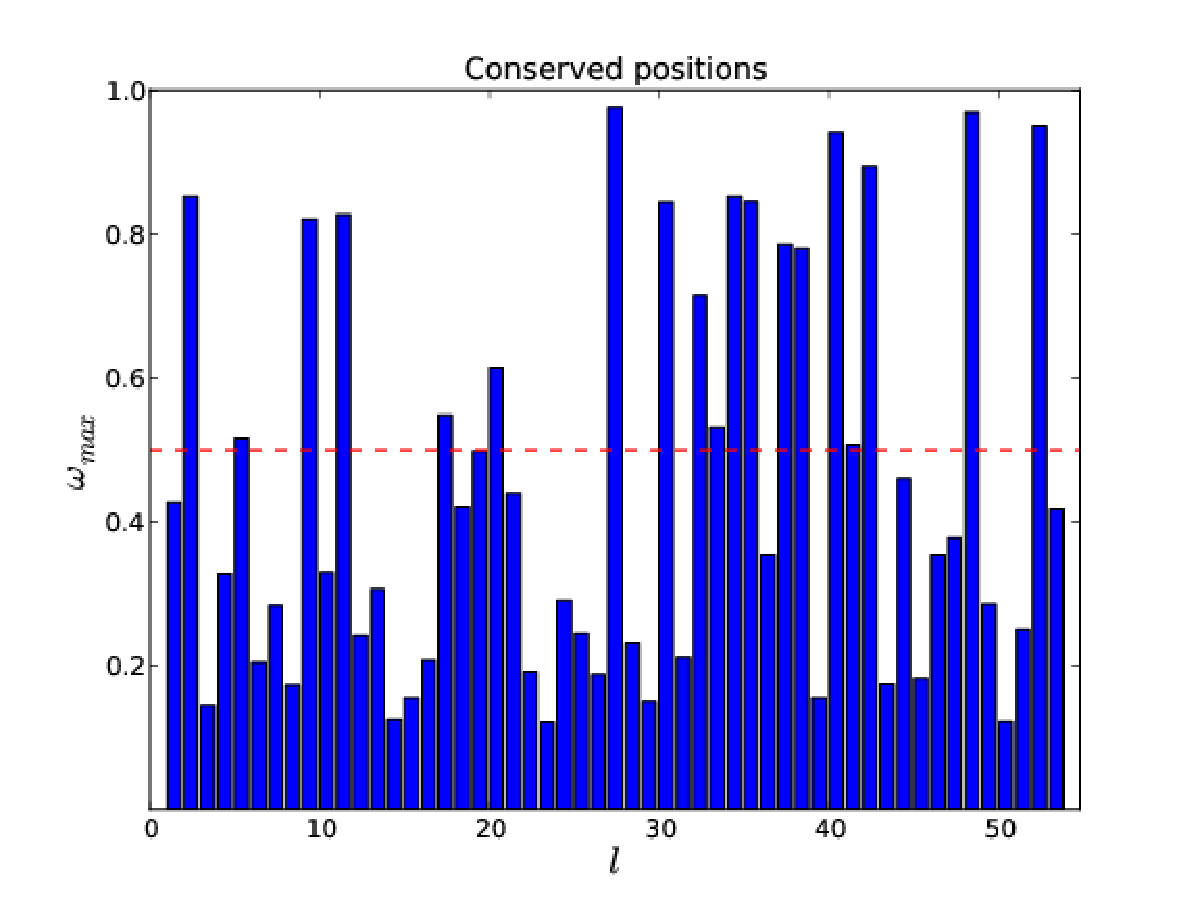
\includegraphics[width=0.5\textwidth]{1.pdf}
%\caption{\label{fig:1}The dotted red line corresponds to $\omega=0.5$. The positions whose bars are above 0.5 are the conserved positions.}
%\end{wrapfigure}

\begin{figure}[b]
\centering
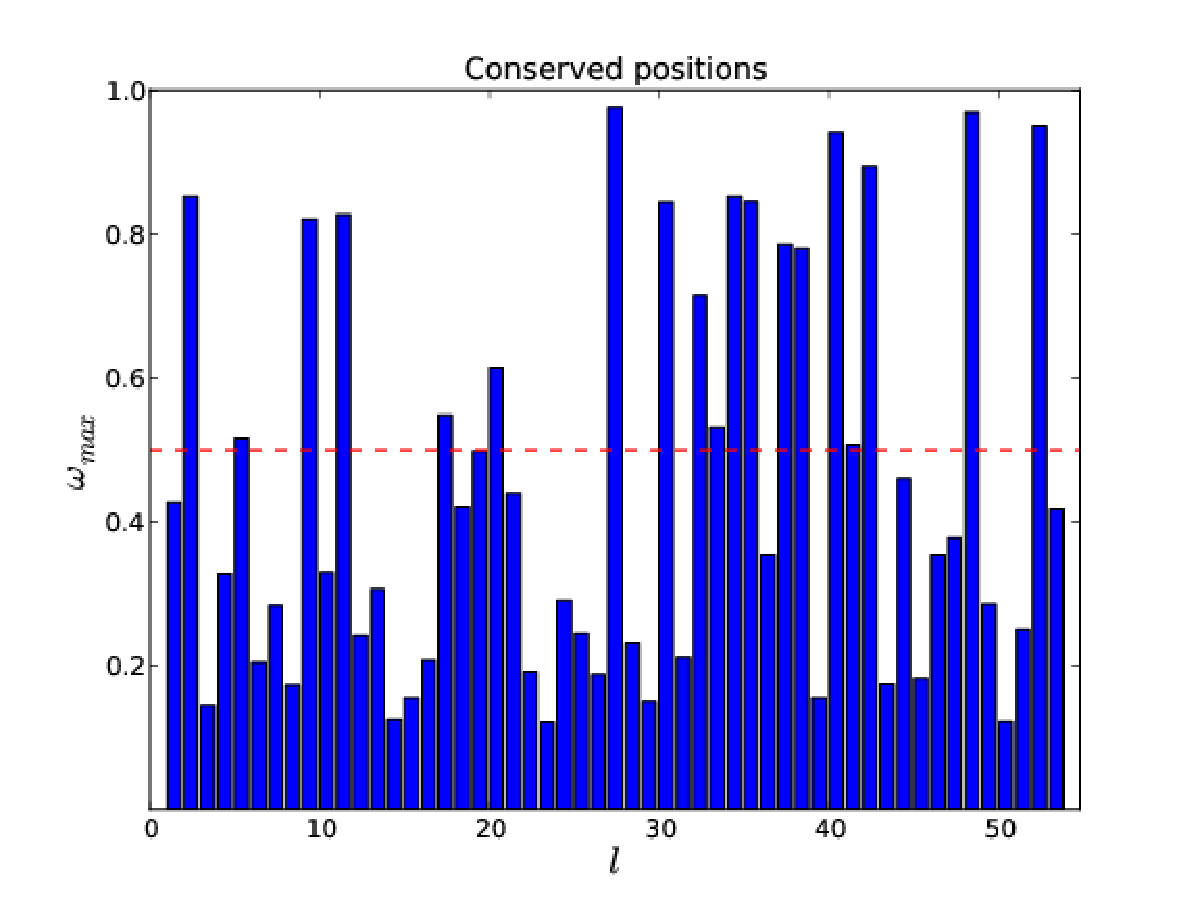
\includegraphics[width=0.49\textwidth]{1.pdf}
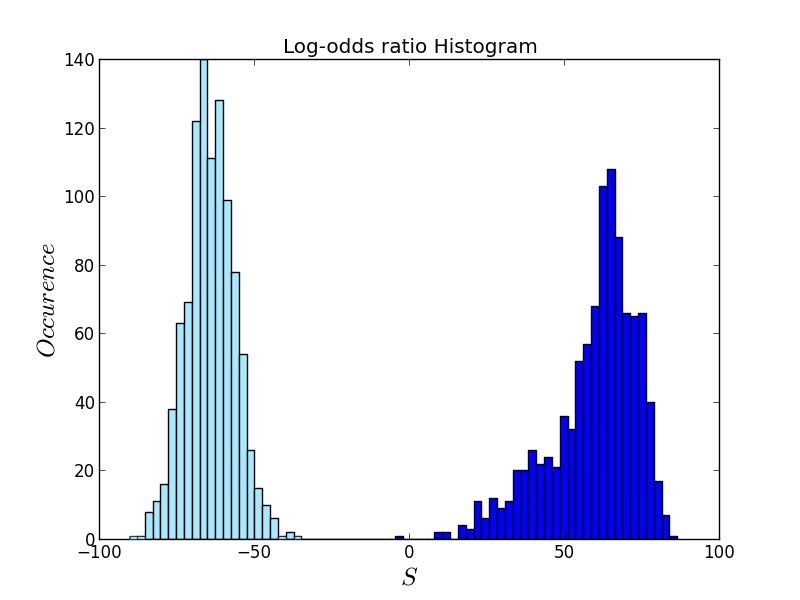
\includegraphics[width=0.49\textwidth]{4.png}
\caption{\label{fig:1}(Left)The dotted red line corresponds to $\omega=0.5$. The positions whose bars are above 0.5 are the conserved positions. (Right) The histogram on the left shows the log-odds ratios for the dataset in the file ``test1.faa'', while the one on the right corresponds to the log-odds ratios of the dataset in the file ``test2.faa''.}
\end{figure}

The three files contain 1000 sequences of 53 amino acids. They are expressed by 20 relevant letters (``A'', ``C'', ..., ``Y'') and few unrelevant letters (``B'', ``X'', ``-'', ect.). In order to analyse the data, we have converted the relevant letters into numbers from 1 to 20 and the unrelevant letters into the number 21. We have then used the data of the file ``train.faa'' that contains the known sequences to construct our statistics.

After computing the probability $\omega_{\ell}(a)$ of the occurrence of an amino acid $a$ in position $\ell$ of the sequences, we select the maximum $\omega_{\ell}(a^*)=\omega_{max}$ for each position and plot it as a function of $\ell$ (see fig.~\ref{fig:1} \emph{(Left)}).

The positions where $\omega_{max}>0.5$ are considered to be \emph{conserved}, i.e. the same amino acid is present along more than $50\%$ of the sequences.

%\begin{figure}[h]
%\begin{minipage}[b]{0.58\textwidth}
%\centering
%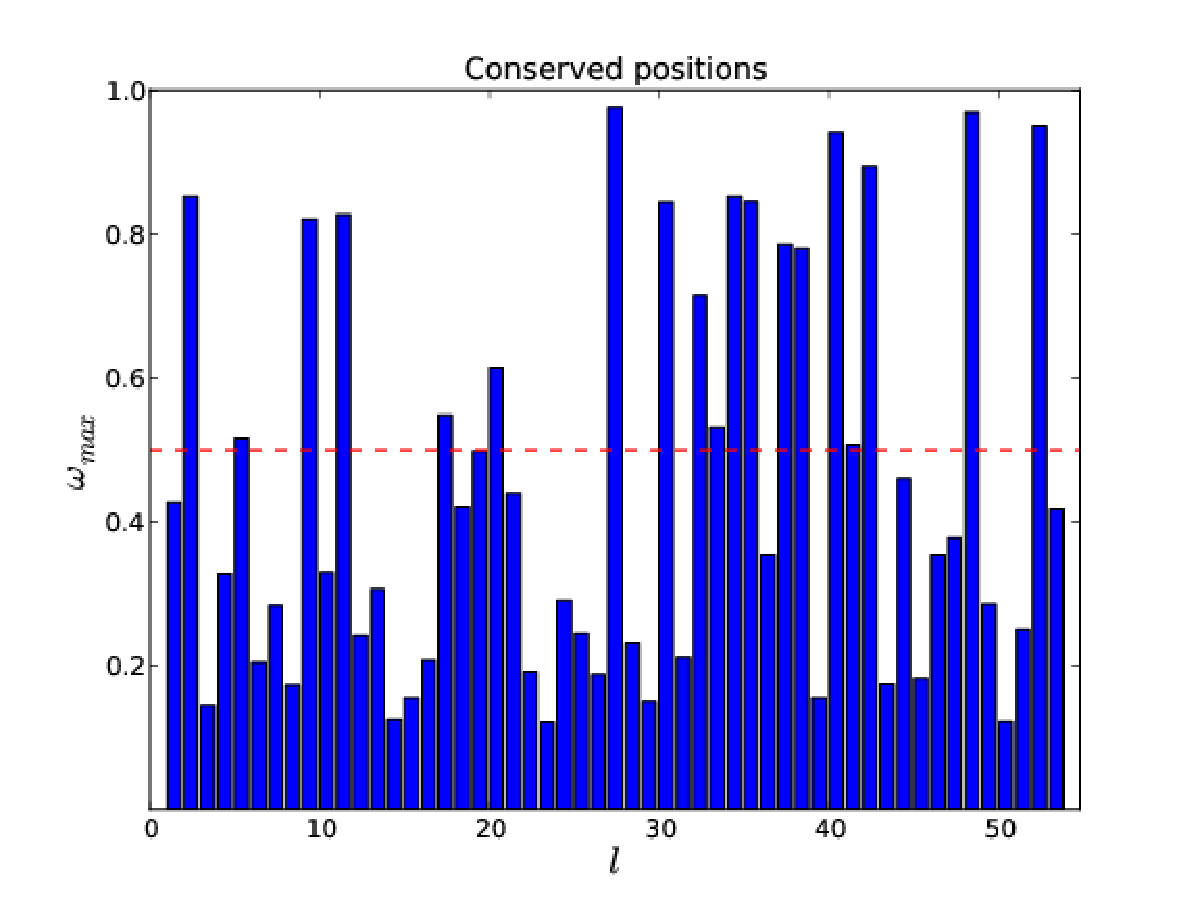
\includegraphics[width=\textwidth]{1.pdf}
%\captionof{figure}{\label{fig:1}The dotted red line corresponds to $\omega=0.5$. The positions whose bars are above 0.5 are the conserved positions.}
%\end{minipage}
%\hfill
%\begin{minipage}[b]{0.39\textwidth}
%\centering
%\begin{tabular}{c c c}
%  \hline
%  Position ($\ell$) & Amino acid ($a^*$) & $\omega_{\ell}(a^*)$ \\
%  \hline
%    2 & 2 & 0.85 \\
%    5 & 13 & 0.51 \\
%    9 & 6 & 0.82 \\
%    11 & 2 &  0.83 \\
%    17 & 15 & 0.54 \\
%    20 & 20 & 0.61 \\
%    27 & 2 & 0.98 \\
%    30 & 5 & 0.84 \\
%    32 & 20 & 0.71 \\
%    33 & 6 & 0.53 \\
%    34 & 6 & 0.85 \\
%    35 & 2 & 0.84 \\
%    37 & 6 & 0.79 \\
%    38 & 12 & 0.78 \\
%    40 & 12 & 0.94 \\
%    41 & 12 & 0.51 \\
%    42 & 5 & 0.89 \\
%    48 & 2 & 0.97 \\
%    52 & 2 & 0.95 \\
%  \end{tabular}
%\captionof{table}{\label{fig:2}Conserved amino acids in conserved positions.}
%\end{minipage}
%\end{figure}




\section{\textbf{Family belonging}}

%\begin{wrapfigure}{r}{0pt}
%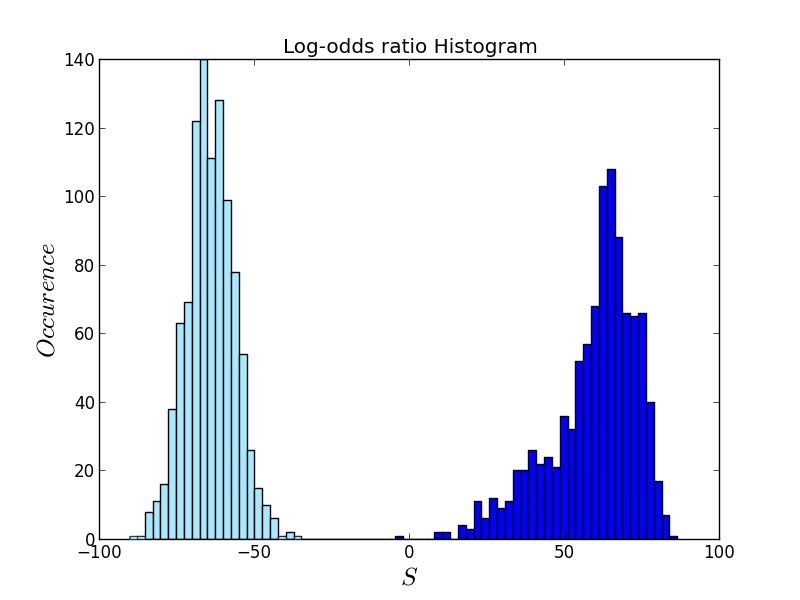
\includegraphics[width=0.5\textwidth]{4.png}
%\caption{\label{fig:3}The histogram on the left shows the log-odds ratios for the dataset in the file ``test1.faa'', while the one on the right corresponds to the log-odds ratios of the dataset in the file ``test2.faa''.}
%\end{wrapfigure}

%\begin{figure}
%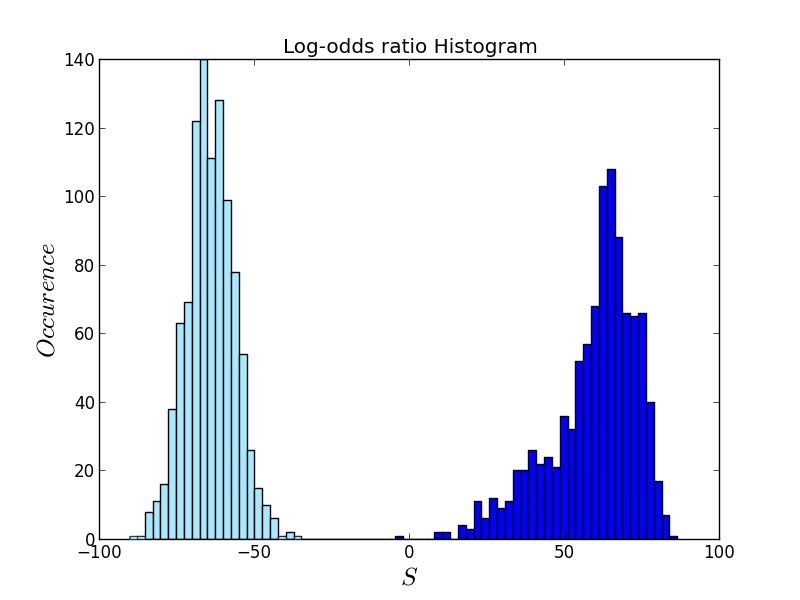
\includegraphics[width=0.5\textwidth]{4.png}
%\caption{\label{fig:3}The histogram on the left shows the log-odds ratios for the dataset in the file ``test1.faa'', while the one on the right corresponds to the log-odds ratios of the dataset in the file ``test2.faa''.}
%\end{figure}

In the previous part we defined the PSWM matrix $\omega_{\ell}(a)$ which characterizes the family of sequences of the dataset ``train.faa''.
The aim of this part is now to determine which dataset between ``test1.faa'' and ``test2.faa'' belongs to the same family of ``train.faa''.
In order to do this we use the method of the log-odds ratio, based on the assumption that amino acids in different positions have no correlations between each other (see fig~\ref{fig:1} \emph{(Right)}). When the log-odds ratios of one set of sequence are positive (negative), it does (does not) belong to the same family of the set in ``train.faa''. 

It is clear that the file that contains sequences that belong to the same family of the ones in ``train.faa'' is ``test2.faa''. What we observe is that the histogram on the left (belonging to another family) is very peaked and symmetric, which means that the sequences are coherent within the same set. On the other hand, the histogram on the right is less peaked and has a longer tail going towards zero: it means that the sequences in that set belong to the same family but are more different between each other.




%%%%%%%%%%%%%% YOUR IMAGE %%%%%%%%%%%%%%%


\section{\textbf{Co-evolution of contact residues}}



Co-evolution between two positions, which are in contact in the folded 3D structure, induces correlations in the amino acid occurrences in these positions. The aim of the last part is to detect these correlations and check if they correspond to a contact in the 3D structure by comparing them with the values in the file ``distances.txt''.

In the figure 3.1 the two colors correspond to the different datasets that were investigated.
From the graphs we can see that for the first $2^2$ pairs the fraction of true-positives is 1, which can be expected since the mutual information of these pairs
is the highest. Beyond $2^5$, the trend in the fraction of true-positives is strictly decereasing, which corresponds well with the fact that these pairs are less
correlated as their rank decereases. What we do not expect is the dip around $2^4$ number of pairs, which we can attribute to the presence of false-positives.
This is comfirmed by the fact that in both datasets we see that the fraction slightly recovers at $2^5$. 




\begin{figure}
\centering
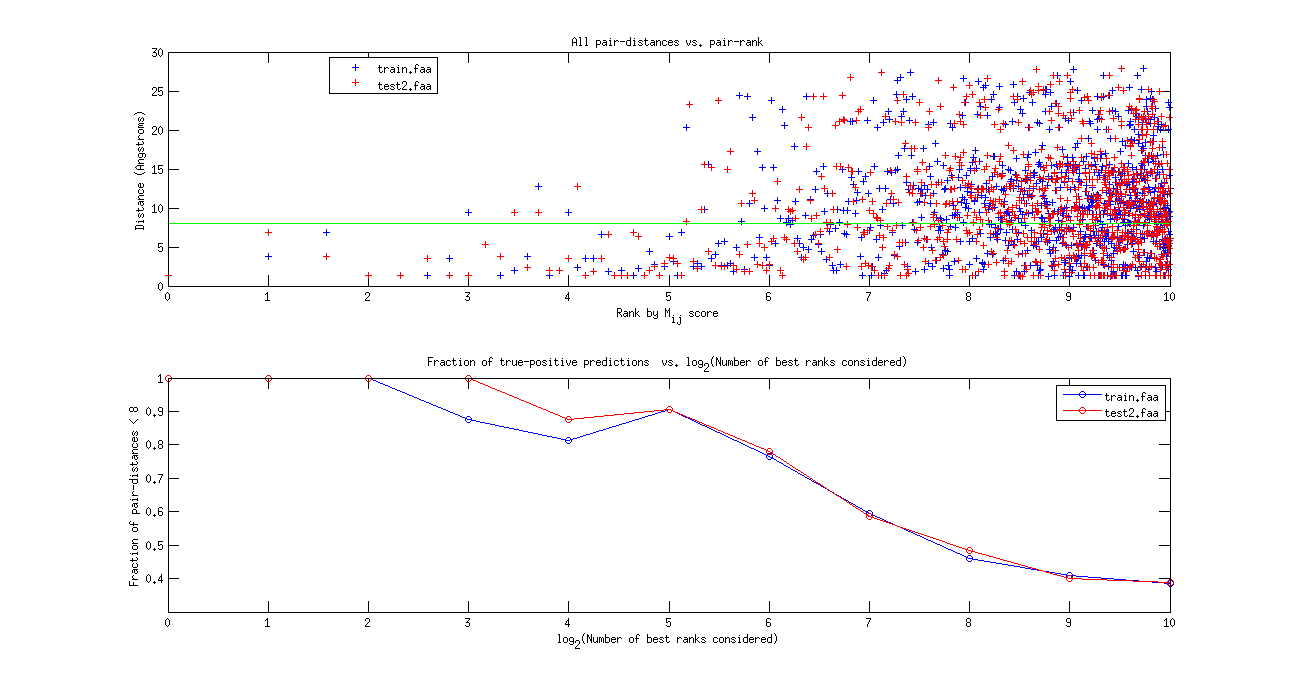
\includegraphics[width=\textwidth]{Results.png}
\caption{\label{fig:4}  
\emph{(Top)} All of the distances are matched with their respective pairs and plotted by their rank depending on their score in $M_{ij}$. The green line denotes the
boundary for distances less than 8 Angstroms. \emph{(Bottom)} The fraction of pair-distances succesfully matched plotted against the number of pairs considered as increasing powers of 2. 
}
\end{figure}

\end{document}
